\section{Sentiment Analysis}
The cornerstone for this thesis is sentiment analysis and this topic requires the definition of a lot of terms and concepts that are important to the research at hand.
Sentiment Analysis in theory sounds rather simple, process text and pull out the meaning based on the content of what was processed, but there are many intricacies that need to be addressed to fully understand the entire process [\cite{liu2012sentiment}].

\subsection{Definition}
Sentiment Analysis refers to the use of natural language processing and text analysis to systematically identify, extract, quantify, and study affective states and subjective information [\cite{liu2012sentiment}].
Sentiment Analysis has increased in popularity in recent years and is popular to use to review large sets of review / survey data to abstract major topics of conversation and controversy online.
It can be an effective tool in summarizing a population's opinions and feelings towards certain issues and drawing conclusions from them.
A basic task of sentiment analysis that can be leveraged into more complex tasks is determining the polarity of a sample of text data and classify it as positive, negative, or neutral [\cite{wilson2005recognizing}].
The process behind sentiment analysis is important and can be complicated depending on how much information an analysis is trying to pull and how large of a dataset is involved, and before the process is addressed, there are certain principles and topics involved that need to be covered first.

\subsection{Natural Language Processing}
Natural Language Processing (NLP) is an important concept that is used heavily in sentiment analysis.
NLP is primarily concerned with the interactions between human beings and computers and specifically how they process and discern the meaning of human language [\cite{liddy2001natural}].
Natural Language Data is abundant in our world today in the Age of the Internet and the vastness of it makes NLP extremely important to implement effectively to aid in understanding this large dataset.
NLP takes on the difficult task of processing large text data and attempting to quantify the text data in different ways.

\subsubsection{Natural Language Toolkit}
NLP is the concept and the implementation in this project is the Natural Language Toolkit (NLTK), which is a Python library that offers NLP methods to process text and extract meaningful trends and patterns from the text of interest.
The NLTK is implemented using Python, which is a simple, yet powerful language with excellent functionality for processing linguistic data \cite{bird2004nltk}.
Much of the meaning is derived using the NLTK but much of the processing is conducted in purely Python using lists of words to process meaning and sentiment.
The task of processing text data comes with a few obstacles that can either obstruct meaning or complicate the processing by changing the meaning of words or phrases based on the context in which they reside.

\subsection{Complications with Text Data}
Text Data can be especially difficult to deal with and cause a lot of unforeseen issues when it is being processed.
The inherent subjectivity of human language and speech is one of the largest obstacles that must be addressed when dealing with any text-based data.
Much of the communication between human beings is subjective and it is up to the interpretation of the speaker and listener what the message is and they can have conflicting ideas on the meaning of some terms [\cite{aggarwal2012mining}].
This potential for miscommunication is mirrored in NLP in that the determined meaning or value of some textual data could not be representative of the source it came from, and there is not an objective reference to the weight of words to confirm the correctness of any one interpretation of the textual data.

Another important factor to consider when processing text data is sarcasm, which is extremely difficult to detect.
Americans especially are known for their use of sarcasm and it can be sometimes impossible to parse such meaning out of text since the intonation is what indicates the sarcasm which is lost in purely text-based data.
There are some subtle cues that can indicate sarcasm in text but it can really only consistently be caught if it is tagged as such [\cite{riloff2013sarcasm}].

A third and final complication that often arises is considering the context in which the text resides [\cite{aggarwal2012mining}].
Context is everything when examining how people speak and trying to accurately access the thoughts and opinions of the speaker so it is important to take this context into consideration when developing a sentiment analysis since it will affect any results that are achieved.
Context here meaning the modifying words surrounding the word to be examined next in the analysis.
Each word in a sample of text data can have any number of modifiers that can manipulate its meaning and fundamentally change what message it is conveying by adding certain words before or after the word.
These modifiers can take on the form of intensifiers, such as very, that amplify the meaning of a word, 

\subsection{Lexicon}
There are several ways to conduct sentiment analysis, some of which do not require a lexicon but this research used a lexicon-based approach.
An important tool that is necessary in conducting this analysis is a comprehensive lexicon.
A lexicon is a database of words and accompanying features associated with each word [\cite{taboada2011lexicon}].
These features associated with each word vary widely in what they say about the word, from part of speech to length to polarity score.
The lexicon used in this research consists of a word and an associated sentiment score that is on the scale from -1.0 (negative) to 1.0 (positive), indicating how positive or negative the word is.
These sentiment scores were compiled from several different lexicons and the results were compiled by surveying thousands of individuals and having them score a certain subset of words and combine those ratings into an average score for each word [\cite{somasundaran2010lexicon}].

\subsection{Alternative Sentiment Analysis Approaches}
There are other ways of conducting sentiment analysis without the use of a lexicon that can also be useful for conducting the analysis.
The main alternative method is a comparative approach that compares each block of text data to one another and instead of giving them an objective score, ranks them according to a subset of rules that determine their ranking relative to the other samples of text [\cite{wilson2005contextual}].
This approach puts much more focus on the context of what is being said and uses context to determine the polarity of language.
This is the main approach used by many political science researchers, since it is far easier to compare politician's values relative to one another than use an objective dictionary to determine their stance on an issue. [\cite{laver2003extracting}]

\subsection{Process}
The process behind sentiment analysis, especially when it is lexicon-based, is rather simple to understand but there are a lot of hidden factors that must be considered.
The most important and most influential part of this entire process is the lexicon, which was covered in the previous section.
The lexicon is used as the basis for all the sentiment scores that are assigned in the analysis, thus its integrity and accuracy is central to the success of the analysis.
The analysis is started by feeding in the text data to the program. 
In this case, that text data was the Presidential State of the Union Addresses.
This text data is split into an array, each index corresponding to an individual word.
At this point, the text data is cleaned up, using assorted algorithms to handle punctuation and capitalization and other linguistic features that could complicate the sentiment score assignment.
Once the data is cleaned, it is time to start the bulk of the sentiment score operation.
Using nested for-loops, each individual word is compared to a list of "common" words to avoid wasting time and processing power on "the" and other non-notable words, and then each non-common word is compared to the lexicon the score for that individual score is recorded in an overall score variable.
As each word is processed, this score variable is either incremented or decremented based on the value associated with said word in the lexicon, and also an overall counter variable is incremented each time, counting each individual word.
After all the words have been processed, the total score that has been tabulated is then divided by the counter and that resulting number is the sentiment score for that selection of text.
There are a couple of odds and ends that were glossed over that will be covered in the next sections since they were added after the initial algorithm was constructed that slightly influence it's behavior when encountering certain specialty words, and also classifying different topics within the body of text.

\begin{singlespace}
\begin{algorithm}[H]
\DontPrintSemicolon
\KwIn{All State of the Union Addresses}
\KwOut{The sentiment score for each Presidential Address for each category.}
\BlankLine
open all .txt files and store them in lists of special category trigger words\;
\For{each address in the State of the Union Addresses}
	{format address\;
	split address in to sentences\;
	\For{each sentence in the address}
		{add sentence to 'overall' category\;
		\If{sentence contains category trigger word}
		{add sentence to category}
	\For{each category}
		{append list of sentences for that category to an overall list}
	\For{each topic in the overall list}
		{\For{each word in the topic}
			{create word count for each word and store it in a dictionary\;
			\If{previous word negator}
				{increment negator counter for that word by one}
			\If{previous word intensifier}
				{increment intensifier counter for that word by one}
			}
		\For{each word in the dictionary}
		{\If{word is in lexicon}
		{\If{length of negators[word] != 0}
		{Subtract length from total count for that word}
		}
		\If{length of intensifiers[word] != 0}
		{Raise length number of scores to the power of 2}
		Calculate the Sentiment Score by multiplying the number of occurences of the term by the score in the lexicon.
		}
		}
	}
	}
	
\caption{Sentiment Analysis Algorithm}
\label{alg:one}
\end{algorithm}
\end{singlespace}

\subsection{Scatter Plot}
Scatter plots are effective at showing data over time and it allows for users to see overall trends in tone and compare the scores across presidencies to see tonal shifts over a president's tenure or how two presidents compared to one another.
The data set lends itself to this representation and the result is a nice longitudinal summary of presidential tones over the course of history and you can see this scatter plot in Figure \ref{fig:scatterplot1}.
The data being displayed isn't objective and it must be taken with a grain of salt because sentiment analysis is far from an exact science and the lexicon is objective but also doesn't take in to account the change of meaning seen in some words.
The time period for these changes is a relatively short period of time in the context of language so the differences shouldn't be greatly significant in the shifting of tone but it is something to note.
The scatter plot itself also allows for interaction in that the user can hover over a point and get detailed information about it, such as the President's name, the term and year that address was delivered, as well as the exact sentiment score.
Figure \ref{fig:scatterplot2} shows the hover feature over a specific Presidential address and showing the detailed information of the president's name, number, party, and sentiment score.
Figure \ref{fig:scatterplot3} shows the other hover feature wherein if a user hovers over a President's name then it shows all of their addresses and fades out the rest of them.
Figure \ref{fig:scatterplot4} shows a different scatter plot with the same data but color coded based on a president's political party to show different trends that follow political party lines.

\begin{figure}
  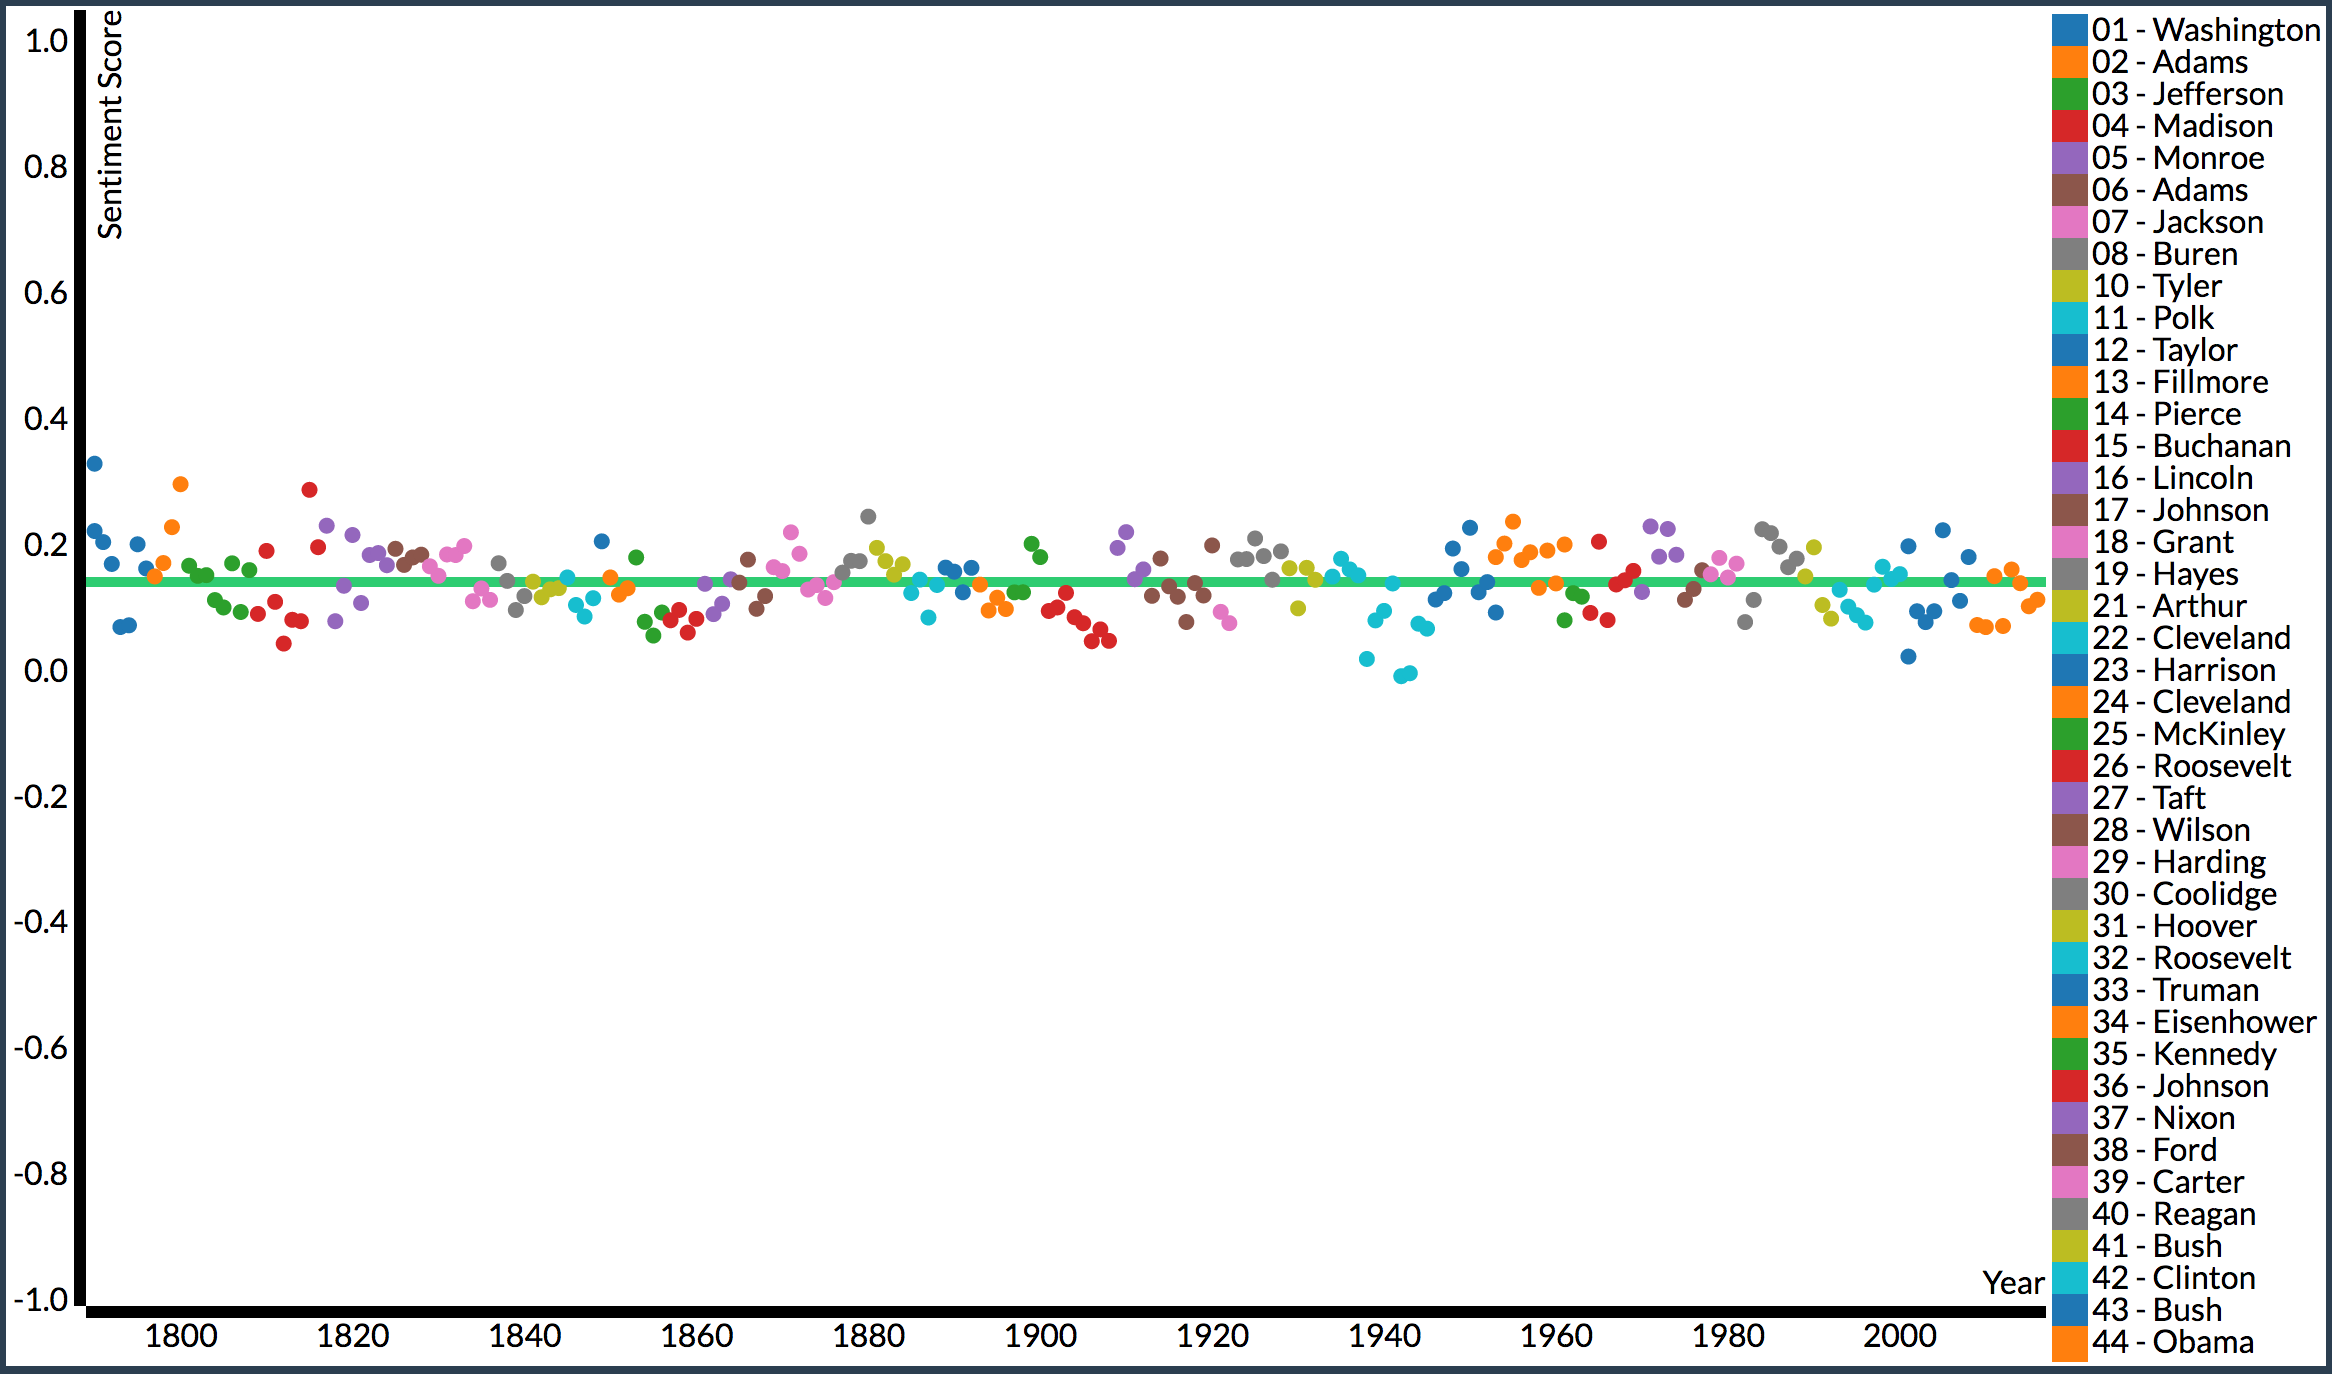
\includegraphics[width=\columnwidth]{images/scatter_plot.png}
  \caption{Scatter Plot}
  \label{fig:scatterplot1}
\end{figure}

\begin{figure}
  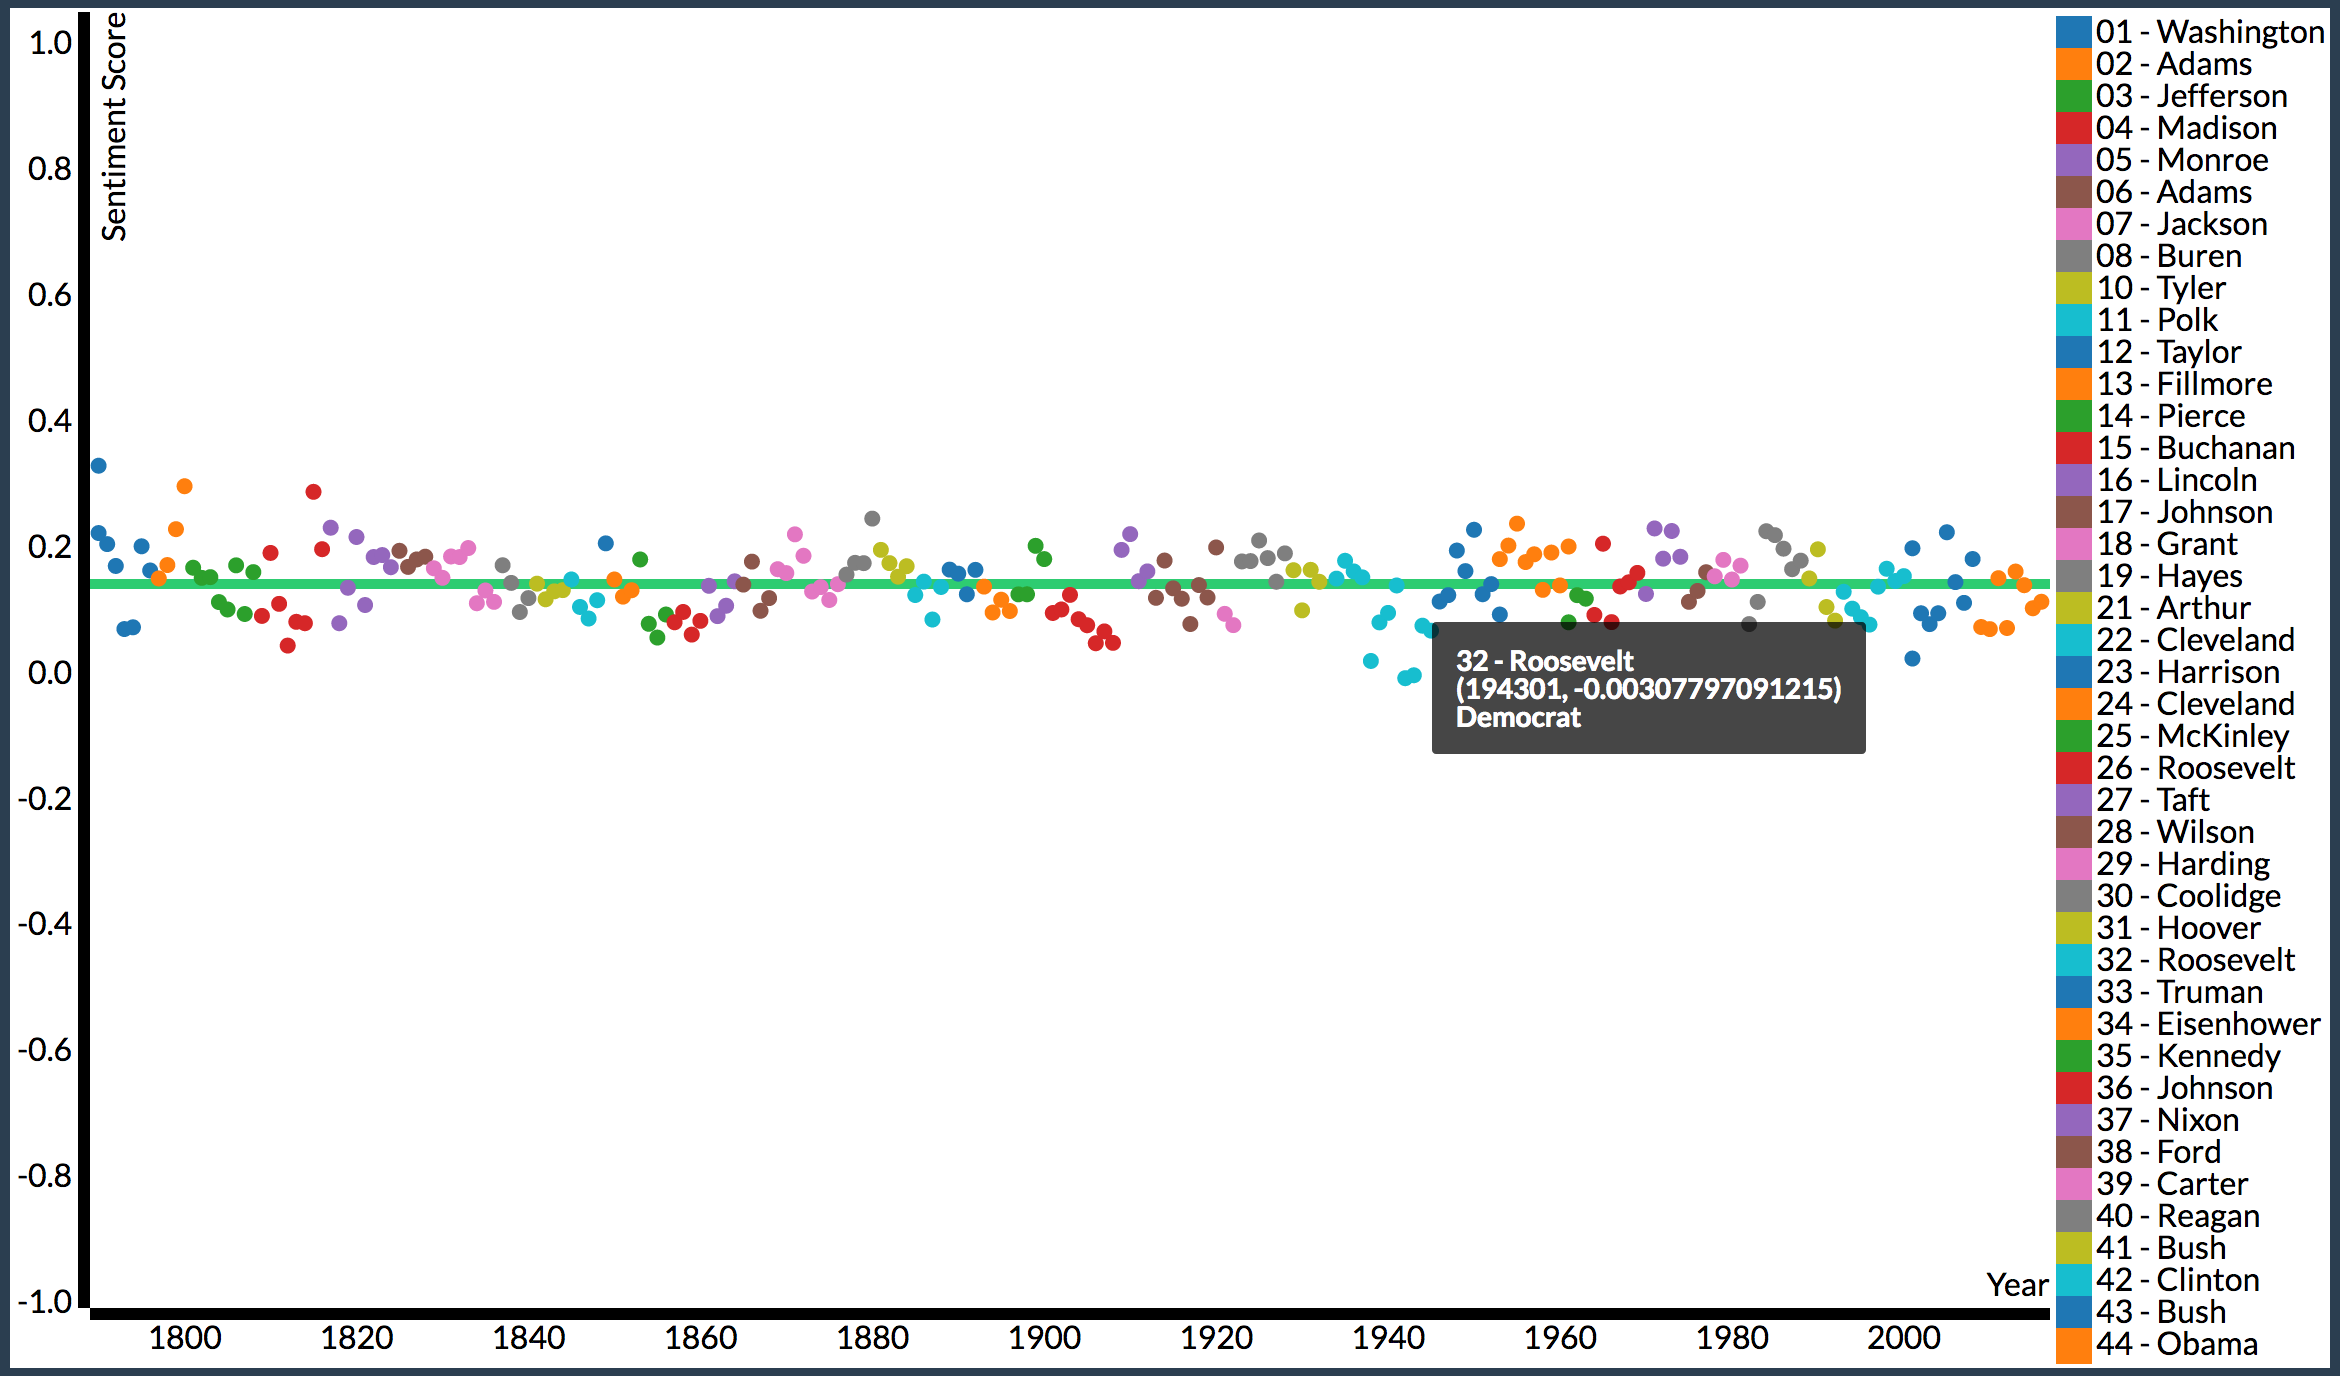
\includegraphics[width=\columnwidth]{images/hover_address.png}
  \caption{Scatter Plot (Hover over Address)}
  \label{fig:scatterplot2}
\end{figure}

\begin{figure}
  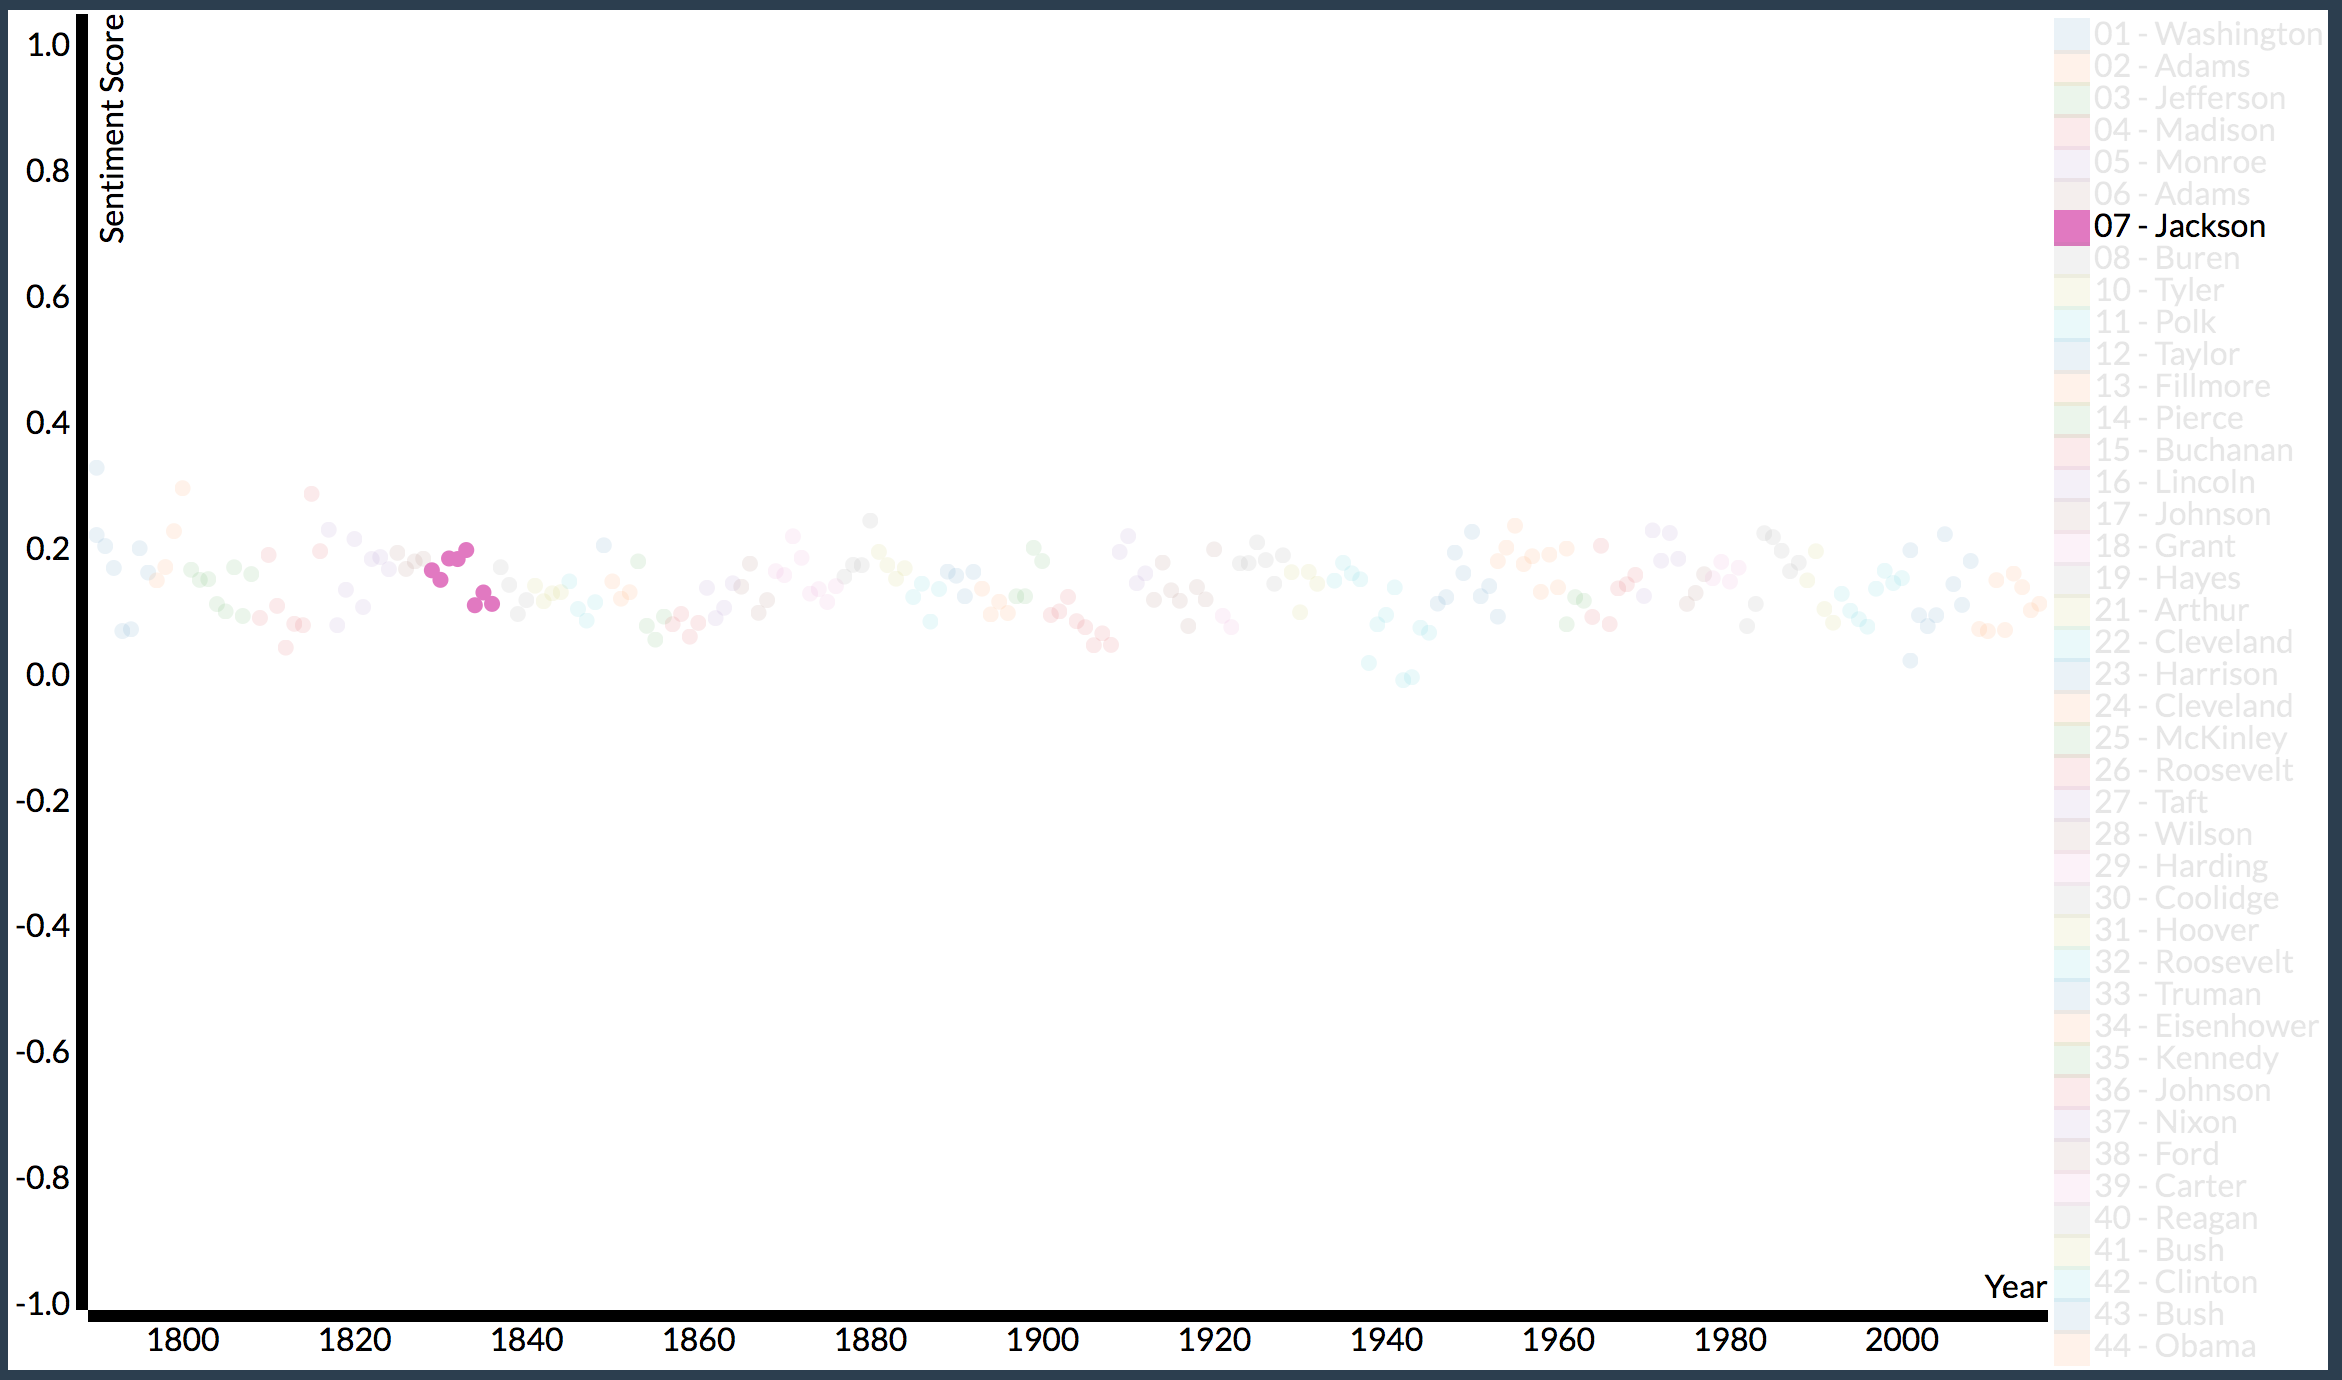
\includegraphics[width=\columnwidth]{images/hover_president.png}
  \caption{Scatter Plot (Hover over President Name)}
  \label{fig:scatterplot3}
\end{figure}

\begin{figure}
  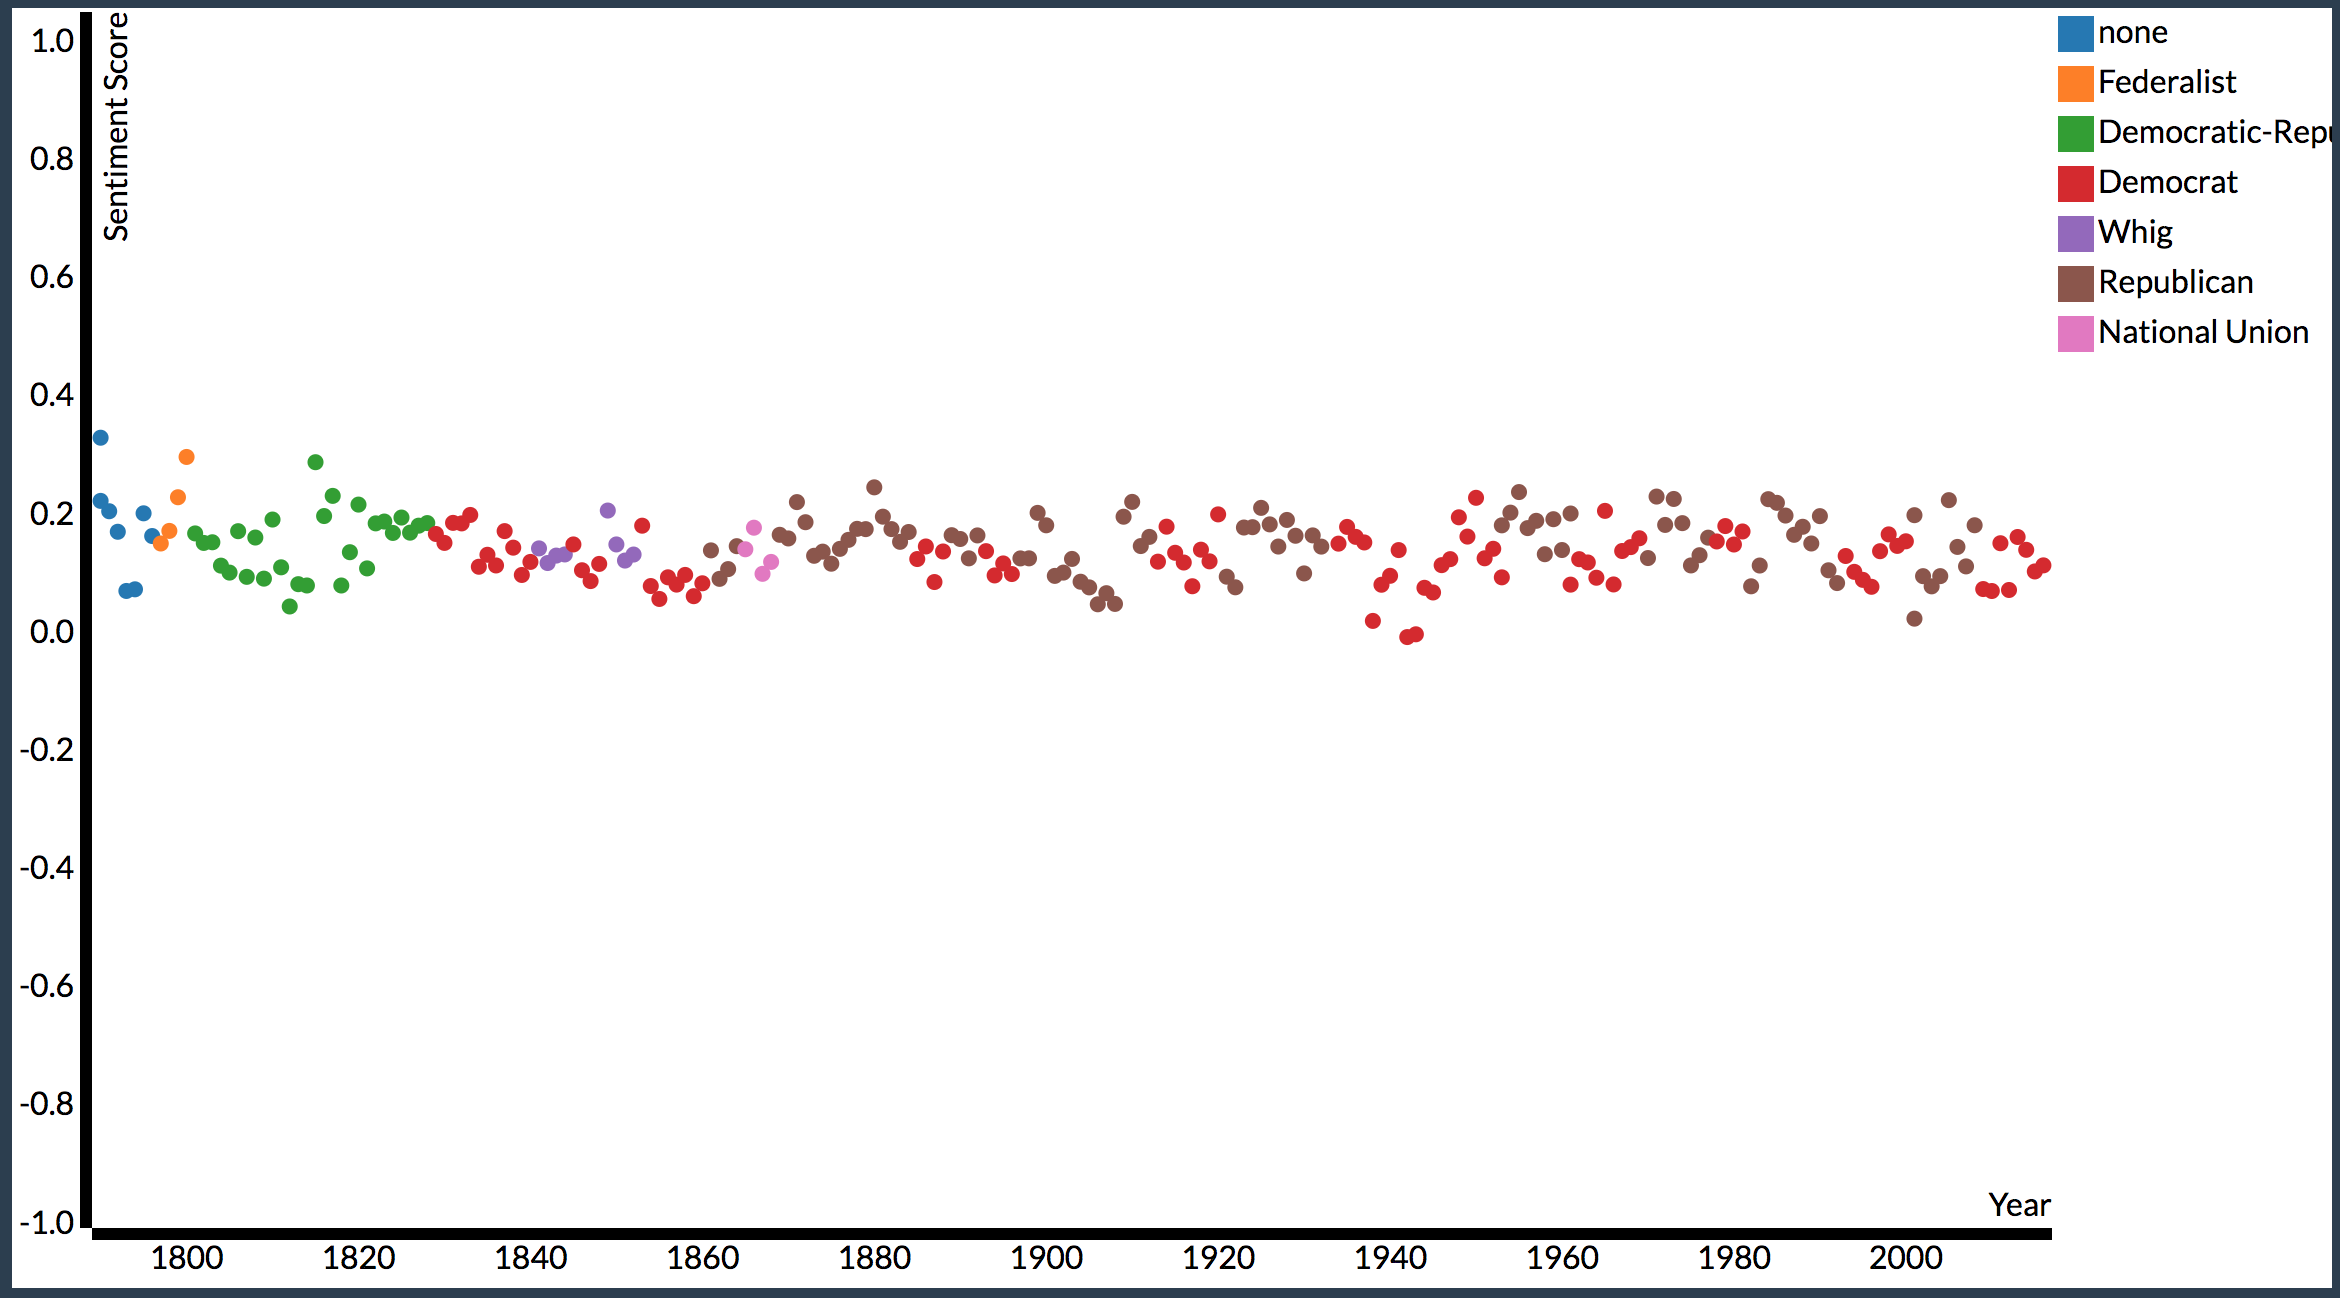
\includegraphics[width=\columnwidth]{images/scatter_plot_party.png}
  \caption{Scatter Plot Party Comparison}
  \label{fig:scatterplot4}
\end{figure}

\subsection{D3}
D3.js (D3) is the JavaScript Library used to create the two visualizations mentioned in the previous sections.
This tooltip functionality was used in the line plot demonstration mentioned previously to give extra information on each data point without cluttering the visualization itself.
Another feature implemented using D3 is that if the user hovers over a President's name, then just that President's data points will be highlighted and the rest are faded out of the screen.

\section{Results}
This sentiment analysis is important to consider when analyzing the addresses and produces some interesting trends to dissect and investigate.

\subsection{Overall}
Generally, the trend for all addresses is that they hover around 0.00 to 0.30 sentiment score, which is telling of the general approach and purpose of the State of the Union Address.
The address is used to convey the problems and issues that are impacting the country, and also to inspire hope that the country is making progress and that it is thriving, which has more of the emphasis.
This slightly positive average overall describes an overall positivity among the presidents in their address to the United States citizens to inspire hope and confidence while also tending to the negative aspects of their presidency to show that change will be made.

\subsection{Presidential Tone Trends}
There are some interesting trends to examine in the tone of each president over time during their presidency.
The overwhelming trend tends to be a generally positive tone for the early addresses that gives way to a more negative tone as the stark realities of the presidency become more apparent and the frustrations of being President start to show their effect in their speeches.
This trend does have some notable exceptions, with John Adams, Rutherford Hayes, and George Bush starting lower and expressing more positive sentiment throughout their Presidential addresses.
George Bush is most likely caused by 9/11 and the lingering effects that it had on his outlook on the presidency and the world at that time, but he got generally more positive over the course of his addresses following 9/11.

\subsection{Historical Events}
A large compounding factor that can have a heavy-handed influence on presidential addresses are major historical events such as the Civil War, the World Wars, the Great Depression, and 9/11.
These events were dark and negative and it is interesting to examine the general tone of the Presidents during these times to see how they approached these grave and serious topics.
They could be very realistic and tell it like it is to be frank with the American people, or merely address the elephants in the room, but still espouse positivity to boost the morale of the country to keep them dedicated to whatever cause it is that they are fighting.
The overall trends in positivity versus negativity that could have many compounding factors that can't be fully investigated without a full psychological breakdown of each of the presidential candidates.
As such, the main consideration here is historical events since they are more outwardly facing and its easier to examine their external effects on the United States and the Presidency than examining the preconceptions and biases felt by each president.
These trends do mirror closely to negative events coinciding with the addresses at the time, indicating the sensitivity of the Presidential outlook to major historical events.
This isn't as true in the case of the Civil War as there aren't any major dips in President Lincoln's speeches, likely due to the fact that it was Americans fighting Americans and his role was to attempt to unite the two sides into one cohesive unit so he attempted to avoid any accusatory and divisive language.

An interesting data point to draw attention to is that of FDR's two State of the Union addresses in 1942 and 1943, the only two Presidential Addresses to have a negative sentiment score in the entirety of the State of the Union's history, -0.01 and -0.005, respectively.
This negativity shows signs of the hard times that was befallen during that time period in American History.
FDR led the United States through the Great Depression, as well as World War II, and he won four presidential addresses, so the people respected him and his word [CITE].
FDR was comfortable in his position in power and used this solidified power to talk frankly to the American People about the dark times that were surrounding them.
World War II was one of the most tragic events to befall this entire world and the tone of the President, and thus, the United States, reflects that.

Another interesting data point to pull out is that of George Bush's September 2001 Address, shortly after 9/11 had occurred.
This was not a State of the Union address in the historical sense but it was needed given the events that had transpired so it is considered to be one.
The overall negative sentiment score of this address (0.02) when compared to his generally positive other addresses shows the dark and serious times that were apparent in these times.
George Bush addressed the people with sorrow and remorse and this language and purpose reflected itself in the tone of the words he chose to use in this address.
This sadness, coupled with the calls for military action against the perpetrators of this tragedy tinged this address with negative and spiteful feelings, making it the third most negative address, and being an extreme outlier in Bush's sentiment scores.

A third and final interesting point to examine is that of the very first State of the Union Address by George Washington in January of 1790.
It is intriguing that the first State of the Union Address is actually the most positive of the entirety of the United States but from a sociological and historical perspective it does make sense.
The United States is a young country and was in the state of being a democratic experiment since nobody knew if it would actually work [CITE - dem experiment].
It took George Washington as the leader of this young nation to inspire hope and foster confidence in this new country that it will succeed and democracy will prevail.
An important role that he didn't take lightly, as can be seen by the overwhelmingly positive approach he took to the first State of the Union address.
Analyzing this in conjunction with his other sentiment scores is intriguing as they fall off sharply and he becomes generally more negative throughout his presidency, talking more of the stark realities of successfully building a strong country than the flowery patriotic speech of his first address.
The trend does curl back up into generally more positive territory in his latter two addresses, an attempt to encourage the citizens and those who would assume his office in years to come with the confidence to drive America forward and make this democratic experiment a success.